\chapter{Further work on the model}
\label{secondPhaseOfModelingCyberInsurance} 

So far we have build a model reflecting how the purchase of cyber-insurance can force the formation of insured sub-graphs. As described earlier, the sub-graph would benefit from forming a star network. In this chapter our focus will be to show how we could force the sub graph to form a start topology. 

In the previous models our utility equations has generated payoffs according to a nodes own earnings, in addition to the extra payoff, $\beta$, received when establishing a new connection. To be able to force the creation of a start topology, we need a new approach which allows nodes to increase their payoffs due to positive network externalities when connecting to the same node. Our idea is based on the paper from Jackson and Wolinsky \cite{jackson1996strategic} and a network formation game in \cite{jackson2005survey}. 

\section{The connection game}
The connection game reflects not only the benefit from establishing connections to other people, but also the benefits from indirect connections. Meaning, in addition to the benefit from the direct connection, a node will also benefit from "a friend of a friend", although the benefit will be a factor lower than the direct connection, also "friends of a friend of a friend" will generate benefit and so forth. The payoff will be calculated relative to the distance between different nodes.


\begin{figure}[h]
\centering
  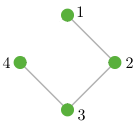
\includegraphics[width=0.2\linewidth]{../Figures/connectionGame.png}
  \caption{\label{fig:connectionGame} Four nodes interconnected with each other.}
\end{figure}
For instance, node 1 in the network depicted in figure \ref{fig:connectionGame}, will benefit $\beta$ from node 2, $\beta^{2}$ from node 3 and $\beta^{3}$ from node 4. The benefit will decrease relative to the shortest path between two nodes as long as $\beta < 1$. Hence the payoff a node receives from the network equals: 

\begin{equation}
\sum_{j\neq i}^{} \beta_{ij}^{d(ij)} - \sum_{j:ij\in g}^{} {I_{l}}_{ij}, 
\label{connecetionGame}
\end{equation}

where $d(ij)$ represents the shortest path between node $i $ and node $j $, and ${I_{l}}_{ij}$ represents node i's cost of insuring a link between the two nodes. To simplify the model we choose a symmetric connection process where $\beta$ and $I_{l}$ is set to a fixed global value. 

To set the conditions for the formation game, one might consider making the network as efficient as possible or focus on creating a stable network. An efficient network means ending up with a network which generates the most total value for the players. Intuitively, this network is preferable if it is stable. However, as we shall see there might be some conflict areas. 

The paper from \cite{jackson1996strategic} showed that the following propositions for a efficient network structure:
\begin{enumerate}
\item a complete graph $g^N$ if $I_{l}<\beta - \beta^2$,
\item a star encompassing every node if $\beta - \beta^2 < i_{l} < \beta + \frac{(N-2)}{2}\beta^2$
\item no links if $\beta + \frac{(N-2)}{2}\beta^2 < I_{l}.$
\end{enumerate}

Generally it means that when the cost of insuring a link is low, it would be more beneficial to have a direct connection to a node than indirectly benefiting from it. When the insurance cost is high, it would not be beneficial to establish connections to others, therefore there will not be created any links. 
The star structure presents the efficient structure for the intermediate costs of insuring links. A star that encompasses every node will minimize the average path length and uses only a minimal number of links. Even though it is the most efficient network for this game, the condition does not result in stable network structure. The reason is because the center node of the star will have to insure every link connected, which generates a huge cost compared to the other nodes. This scenario is quite unfair, since the center node generates a great deal of network externalities for the other nodes, without being compensated. Hence a number of connections to the center node will not be pairwise stable, and the network will not be stable. 

The conditions has to be changed in order to met the requirements for stability, Jackson and Wolinsky presents the following proposition:

\begin{enumerate}

\item a pairwise stable network consists of at most one (non-empty) component,
\item if $I_{l}<\beta - \beta^2$, the unique pairwise stable network will be a complete graph $g^N$, 
\item if $\beta - \beta^2 < i_{l} < \beta $, a star encompassing every node will be pairwise stable, although not unique.
\item if $\beta < I_{l}$, any pairwise stable network which is nonempty is such that each player has at least two links and thus be inefficient. 
\end{enumerate}

As we can see, the conditions for high and low insurance cost results in just about the same effects as with the efficient network structure. In addition, the case of intermediate insurance cost still have some issues. Since $I_{l} < \beta$ every node has to benefit from interconnected nodes, in order to be profitable. When considering the efficient star network, only an empty network will fullfil this requirement. To see this, lets consider a simple graph where one have a center node and four leaf nodes connected to the center. The utility of the center node will be $U = 4\beta - 4 I_{l}$, which will be negative due to the condition. Hence the graph will not be pairwise stable. 

However, the problem lies with the center node, for the other nodes this will be the efficient structure. This information is known to the insurance companies, and could be used to compensate the center nodes for their contribution to creating an insurable topology. 


TODO: 

To analyze the model we need to look at what efficiency is. 
How can we create a stable star topology

plot the different equations and discuss it. plot with real values from the model.

